% -----------------------------------------------
% Template for ISMIR Papers
% 2023 version, based on previous ISMIR templates

% Requirements :
% * 6+n page length maximum
% * 10MB maximum file size
% * Copyright note must appear in the bottom left corner of first page
% * Clearer statement about citing own work in anonymized submission
% (see conference website for additional details)
% -----------------------------------------------

\documentclass{article}
\usepackage[T1]{fontenc} % add special characters (e.g., umlaute)
\usepackage[utf8]{inputenc} % set utf-8 as default input encoding
\usepackage{ismir,amsmath,cite,url}
\usepackage{graphicx}
\usepackage{color}
\usepackage{amsfonts}


\usepackage{lineno}
\linenumbers

\graphicspath{{../Figures/}}

% Title. Please use IEEE-compliant title case when specifying the title here,
% as it has implications for the copyright notice
% ------
\title{The Concatenator: A Bayesian Approach To Real Time Concatenative Musaicing}

% Note: Please do NOT use \thanks or a \footnote in any of the author markup

% Single address
% To use with only one author or several with the same address
% ---------------
%\oneauthor
% {Names should be omitted for double-blind reviewing}
% {Affiliations should be omitted for double-blind reviewing}

% Two addresses
% --------------
\twoauthors
  {First author} {School \\ Department}
  {Second author} {Company \\ Address}

% Three addresses
% --------------\input{ISMIR2021_paper.tex}

%\threeauthors
%  {First Author} {Affiliation1 \\ {\tt author1@ismir.edu}}
%  {Second Author} {\bf Retain these fake authors in\\\bf submission to preserve the formatting}
%  {Third Author} {Affiliation3 \\ {\tt author3@ismir.edu}}

% Four or more addresses
% OR alternative format for large number of co-authors
% ------------
%\multauthor
%{First author$^1$ \hspace{1cm} Second author$^1$ \hspace{1cm} Third author$^2$} { \bfseries{Fourth author$^3$ \hspace{1cm} Fifth author$^2$ \hspace{1cm} Sixth author$^1$}\\
%  $^1$ Department of Computer Science, University , Country\\
%$^2$ International Laboratories, City, Country\\
%$^3$  Company, Address\\
%{\tt\small CorrespondenceAuthor@ismir.edu, PossibleOtherAuthor@ismir.edu}
%}

% For the author list in the Creative Common license, please enter author names. 
% Please abbreviate the first names of authors and add 'and' between the second to last and last authors.
\def\authorname{F. Author, S. Author}

% Optional: To use hyperref, uncomment the following.
\usepackage[bookmarks=false,pdfauthor={\authorname},pdfsubject={\papersubject},hidelinks]{hyperref}
% Mind the bookmarks=false option; bookmarks are incompatible with ismir.sty.

\sloppy % please retain sloppy command for improved formatting

\newcommand{\ChrisEdit}[1]{\textcolor{red}{(#1)}}
\newcommand{\BenEdit}[1]{\textcolor{blue}{(#1)}}

\begin{document}

%
\maketitle
%

\begin{abstract}
    We present ``The Concatenator,'' a real time system for audio-guided concatenative synthesis. Similarly to Driedger et. al's ``musaicing'' (or ``audio mosaicing'') technique, we concatenate a set number of activations within a corpus of audio to re-create the harmonic and percussive aspects of a target audio stream. Unlike Driedger's NMF-based technique, however, we instead use an explicitly Bayesian point of view, where corpus activations are hidden states and the target audio stream is an observation. We use a particle filter to infer the best hidden corpus states in real-time. Our transition model includes a tunable parameter to control the time-continuity of corpus grains, and our observation model allows users to prioritize how quickly the activations shift to match the target. Because the computational complexity of the system is independent of the corpus size, our system scales to corpora that are hours long, which is an important feature in the age of vast audio data collections. Within The Concatenator module itself, composers can vary grain length, fit to target, and pitch shift in real time while reacting to the sounds they hear, enabling them to rapidly iterate ideas. To conclude our work, we evaluate our system with extensive quantitative tests of the effects of parameters, as well as a qualitative evaluation with artistic insights. Based on the quality of the results, we believe the real-time capability unlocks new avenues for musical expression and control, suitable for live performance and modular synthesis integration, which furthermore represents an essential breakthrough in concatenative synthesis technology.
    
\end{abstract}

\section{Introduction}

Concatenative synthesis, or audio mosaicing, is a data-driven approach to arrange granular fragments of audio samples, particularly using data sourced from the spectral-temporal features of a target sound. While granular synthesis systems typically rely on combinations of aleatoric parameterization, deterministic automation, and traditional synthesis modulation to achieve complex and evolving textures from sound fragments, concatenative synthesis algorithms utilize Music Information Retrieval technology to decide parameters such as the index, amplitude, and pitch of each sound fragment. 

Modern music producers are inundated by audio data. Services like Splice offer hundreds of thousands of samples readily available on the cloud, and Kontakt multi-sample libraries can often take up over 10gb of disk space to capture a single instrument. Music Producers generate plenty of their own audio data as well: stems, multi-tracks, long-form recordings, and mix variations account for a large portion of many a music producer's audio collection. Recent software such as XO by XLN Audio, Sononym, and Ableton Live 12 offer automatic organization of audio files based on various tags and descriptors, but these implementations of MIR technology are more utilitarian than creative in their design and application. Meanwhile, concatenative synthesis options remain sparse since its conceptual inception \cite{schwarz2000system}: Reformer by Krotos is designed to create foley designs, apps like Samplebrain and CataRT \cite{schwarz2006real, schwarz2008principles} are lacking in critical musical areas such as pitch tracking, with the more advanced options having limited accessibility for artists, requiring prior knowledge of Max (FluCoMa, MuBu) or Python (Audioguide).

The Concatenator advances concatenative synthesis in 3 major ways: 1) it is capable of accurate harmonic and percussive reproductions from arbitrary corpora 2) in real-time, 3) affording new levels of control and accessibility for users. The speed, ease, and scope of The Concatenator offers a fresh paradigm for music producers to interact creatively with their ever-expanding excess of audio data, leading what we belive is a breakthrough in the field.

\section{Related Work}
\label{sec:relatedwork}
This work stands on the shoulders of giants in Bayesian inference, particle filters, concatenative synthesis, and applied nonnegative matrix factorization (NMF).

\textbf{Driedger's Technique.} From an artistic point of view, the most similar technique to ours is Driedger et al.'s 2015 ``Let It Bee'' concatenative musaicing technique \cite{driedger2015let}, which uses NMF to learn activations of spectral templates in a \textbf{corpus collection} so that their combination will match a \textbf{target} spectrogram. This technique was a fruitful innovation in sound design for electronic music production, as featured heavily on Zero Point by Rob Clouth\cite{clouth2020}, using custom software also authored by Clouth. The algorithm was also implemented in an open source python script in 2018 \cite{tralie2018}, and in Max by the FluCoMa project in 2021 (fluid.bufnmfcross)\cite{flucoma2021}, which made NMF-inspired audio mosaicing accessible enough to contribute towards the production of at least two more albums heavily featuring the technique: Edenic Mosaics by Encanti (2021) \cite{cantil2021} and Hate Devours Its Host by Valance Drakes (2023) \cite{drakes2023}.


We now detail some of the mathematics of Driedger et al.'s technique, as we borrow a few ideas in our work.  Driedger et al. learn $H$ in the equation $V \approx WH$, where $V$ is an $M \times T$ target spectrogram with $M$ frequency bins and $T$ times, $W$ is an $M \times N$ set of $N$ spectral corpus templates that are treated as fixed, and $H$ is a matrix of $N \times T$ learned activations.  For instance, $W$ could be the windows of a collection of buzzing bees and $V$ could be an excerpt from The Beatles' ``Let It Be'' (hence the title).  Driedger et al. use the Kullback-Liebler (KL) divergence loss, an instance of the more general $\beta$-divergence \cite{buch2017nichtnegativematrixfaktorisierungnutzendesklangsynthesensystem}, to measure the goodness of fit of $WH$ to $V$.  This loss function is 

\begin{equation}
\label{eq:klloss}
D(V || WH) = \sum V \odot \log \left( \frac{V}{WH} \right) - V + WH
\end{equation}

where $\odot$, $/$, $+$, and $-$ are all applied element-wise, and the sum is taken over all elements of the resulting matrix.  As Lee/Seung show, choosing the right step size turns gradient descent of Equation~\ref{eq:klloss}, with respect to $W$ and $H$, into {\em multiplicative update rules} that guarantee monotonic convergence.  Driedger et al. keep $W$ fixed to force the final audio to use exact copies of the templates, so only the update rule for $H$ is relevant.  At iteration $\ell$, this is:

\begin{equation}
\label{eq:klhgrad}
H_{kt}^{\ell} \gets H_{kt}^{\ell-1} \left( \frac{ \sum_{n} W_{nk} V_{nt} / (WH^{\ell-1})_{nt} }{ \sum_{n} W_{nk} } \right)
\end{equation}

Crucially, though, Driedger et al. note that the update rules in Equation~\ref{eq:klhgrad} alone will lose the timbral character of the templates in $W$.  They hence disrupt ordinary KL gradient descent by performing several increasingly impactful modifications to $H$ before Equation~\ref{eq:klhgrad} in each step, which are eventually set in stone after $L$ total iterations.  First, they avoid repeated activations to avoid a ``jittering'' effect, allowing a particular activation $k$ to only exist once in some iterval based on where it's the strongest:
\begin{equation}
    \label{eq:driedgerrepeated}
    (H_r)_{kt}^{\ell} \gets \left\{ \begin{array}{cc} H^{\ell-1}_{kt} & H^{\ell-1}_{kt} > H^{\ell-1}_{ks}, |t - s| \leq r \\ H^{\ell-1}_{kt} (1 - \frac{\ell+1}{L}) & \text{otherwise}  \end{array} \right\}
\end{equation}
for some chosen $r$.  They also promote sparsity in a similar way by shrinking all but the top $p$ activations in each column of $H_r$ to create $H_p^{\ell}$.  Finally, they encourage {\em time continuous activations} by doing ``diagonal enhancement,'' or by doing a windowed sum down each diagonal of $H_p$, assuming the columns of $W$ are also in a time order.

\begin{equation}
    \label{eq:driedgertimecontinuous}
    (H_c)_{kt}^{\ell} = \sum_{i=-c}^c (H_p)^{\ell}_{k+i, t+i}
\end{equation}

Since this encourages the algorithm to mash up chunks of $W$ in a time order, it effectively encourages sound grains from the templates than the length of a single window that ordinary NMF would take.  Finally, Drieger at all apply Equation~\ref{eq:klhgrad} to $H_c^{\ell}$ instead of $H^{\ell-1}$ to obtain $H^{\ell}$.

These disruptions remove the guarantee that Equation~\ref{eq:klloss} will be minimized, or that it will even monotonically decrease, but Driedger et al.'s brilliant insight is that the loss function is merely a guide to choose reasonable activations; a sub-optimal fit leaves room to better preserve timbral characteristics.  We take a similar perspective.

\textbf{Driedger Tweaks.} Interestingly, the idea of spectrogram decomposition used for concatenative musaicing goes back to the work of \cite{burred2013cross}.  Beyond that, the authors of \cite{buch2017nichtnegativematrixfaktorisierungnutzendesklangsynthesensystem} provide some improvements to Driedger et al.'s technique, including sidestepping phase retrieval, which we exploit in our work. One issue with Driedger et al.'s technique is the sources have to be augmented with pitch shifts to span additional pitches in the target, increasing memory consumption and runtime.  The authors of \cite{foroughmand2017multi, aarabi2018music} sidestep this by using 2D deconvolutional NMF \cite{schmidt2006nonnegative}.  Specifically, their technique uses the Constant-Q transform, where pitch shifts are modeled as constant shifts of the activations instead of the templates, saving memory.  The other added activation dimension models time history and time shifts to avoid the need for the diagonal enhancement of Equation~\ref{eq:driedgertimecontinuous}.  Interestingly, the authors apply 2D NMF to both the source material and the target, so they do not preserve the original sound grains.  However, for our preferred style, we want to take the source grains exactly as they are.


\textbf{Classical Concatenative Synthesis.} Schwarz created an offline concatenative synthesis system dubbed ``Caterpillar'' that uses the Viterbi algorithm \cite{schwarz2000system}, which he later approximated with a real time system, "CataRT" that uses a greedy approach instead of the Viterbi algorithm \cite{schwarz2006real, schwarz2008principles}.  Simon's ``audio analogies'' is quite similar \cite{simon2005audio}, but instead of a user controlled traversal through timbral space, they use features from some source (e.g. midi audio) to guide synthesis to a target with a different timbre (e.g. real audio of someone playing a trumpet). Caterpillar and audio analogies are both {\em sequentially Bayesian in nature}, where the {\em hidden state} is the template to concatenate, and the ``observation'' is a user-controlled trajectory or features from a source timbre, respectively.  The prior transition probabilities are based on temporal continuity.  However, they use the Viterbi algorithm, which is computationally intensive and which needs all time history, so it cannot be applied in real time.  By contrast, a \textbf{particle filter} is a Monte Carlo method for real time sequential Bayesian inference \cite{metropolis1949monte, doucet2000sequential, thrun2002probabilistic}.  It is less common in MIR, but it has found use in a few real time MIR applications such as multi-pitch tracking \cite{duan2011state}, tempo tracking \cite{cemgil2003monte, hainsworth2004particle}, and beat tracking \cite{heydari2021don}.  

\begin{figure*}[h]
	\centering
	\includegraphics[width=\textwidth]{figs/BlockDGM.pdf}%
	\caption{A block diagram of \textbf{The Concatenator}, which remixes a corpus to sound like a target audio stream in real time.  Each particle captures $p$ corpus activations, each which moves forward by 1 step in time with probability $p_d$, or which jumps to a random corpus position otherwise. Weights are updated based on how well the activations fit incoming audio.   }
	\label{fig:BlockDGM}
\end{figure*}

\section{The Concatenator}



The NMF technique of Driedger is not suitable for realtime applications; the gradient update rules of Equation~\ref{eq:klhgrad} scale quadratically in the length of the corpus, leaving all but minutes long corpora usable (Section~\ref{sec:complexity}), and the equations to promote repeated activations and time continuity at each entry of $H$ require knowledge of all activations in $H$, including future activations.  Instead, The Concatenator does many tiny KL-based NMF problems (Equation~\ref{eq:klhgrad}) online based on random sampling at each timestep, and then has them vote on a final set of activations to use at that timestep (Figure~\ref{fig:BlockDGM})\footnote{Instrument images adapted from \url{vectorportal.com}}.  The random sampling trades off historical context to choose longer grains with fit to the target audio that's streaming in.  We provide the mathematical and implementation specifics below.

\subsection{Sequential Bayesian Formulation And State Space}
\label{sec:bayesian}

    Formally, the The Concatenator uses a sequential Bayesian formulation, viewing the target spectrogram (or some derived feature) $V$ as the observation, where the $t^{\text{th}}$ column of $V$ is an observation at time $t$.  The hidden states is the activations of the $N$ templates in the corpus spectrogram $W$ at each time.  We then use a particle filter to efficiently infer the hidden activations (Section~\ref{sec:sampling}).
    
    Henceforth, we will refer to the observations, or columns of $V$ at time $t$ as vectors $\vec{v}_t$ to emphasize that the data is streaming, and we focus on one timestep $t$ at a time.  
    
    \textbf{State space.} To keep the state space simple, we decouple which activations are active from their weights; we only model the former as the hidden state, while we infer the weights as a best fit under the KL-loss (Equation~\ref{eq:klloss}).  To control for polyphany directly, we use a {\em $p$-sparse} nonnegative integer-valued vector $\vec{s}_t \in \mathbb{Z}^{+p}$ as the hidden state.  This vector indexes the $p$ corpus elements that are active at time $t$, where $p$ is fixed ahead of time.  For convenience of implementation, we allow repetitions of template indices, and the indices are in no particular order:%\footnote{One could also model $\vec{s}_t$ as a \textbf{set} of $p$ elements, which would identify all $\vec{s}_t$'s that are permutations of each other.  This would reduce the cardinality of the state space to $\binom{N}{k}$ at the cost of a more cumbersome implementation.  We also rely on some redundancy sampling good activations in our particle filter, so allowing repetitions does not hurt performance.}:

    \begin{equation} 
        \label{eq:statevector}
        \vec{s_t}[k] \in \left\{0, 1, ..., N-1\right\}, k = 0, 1, ..., p-1 
    \end{equation}

    We then infer the associated nonnegative weights $\vec{h_t}[k]$ for each activation to give the approximation $\vec{\Lambda_t}$ at time $t$:
    
    \begin{equation}
        \label{eq:approximation}
        \vec{\Lambda_t}[n] = \sum_{k} \vec{h_t}[k]  W_{n, \vec{s_t}[k]}
    \end{equation}

    In particular, given $W$, $\vec{s_t}$, and $\vec{v_t}$, we apply the update rules of Equation~\ref{eq:klhgrad} for a pre-specified number $L$ of iterations, using the corresponding columns $\vec{s_t}$ of $W$

    \begin{equation}
        \label{eq:sparseklhgrad}
        \vec{h_t}^{\ell}[k]  \gets \vec{h_t}^{\ell-1} \left(  \frac{\sum_n (W_{n, \vec{s_t}[k]}) (\vec{v_t}[n]) / (\vec{\Lambda_t}^{\ell-1}[n]) }{ \sum_{n} W_{n, \vec{s_t}[k]}} \right)
    \end{equation}
    

    \textbf{Transition Model.} We use the KL-loss (Equation~\ref{eq:klloss}) to measure the spectral fit of $\Lambda_t$ to $\vec{v_t}$, which we'll refer to as $d_t$.  As in Driedger et al. \cite{driedger2015let} (Equation~\ref{eq:driedgertimecontinuous}), however, we are willing to sacrifice fit to take longer grains from the corpus $W$.  To that end, we define the prior  \textbf{state transition probability} in the as a Factorial Hidden Markov Model (FHMM) \cite{ghahramani1995factorial}, where components of each activation transition independently from each other, but they contribute jointly to an observation (Section~\ref{sec:sampling}).  The transition model is as follows:

    \begin{equation}
        \label{eq:transitionprob}
        p_T(\vec{h_t} = \vec{b} | \vec{h_{t-1}} = \vec{a}) = \prod_{k=0}^{p-1} \left\{  \begin{array}{cc}  p_d & b[k] = a[k]+1  \\ \frac{1-p_d}{N-1} & \text{otherwise} \end{array} \right\}
    \end{equation}
    where $p_d \in [0, 1]$ is the ``probability of remaining time-continuous.''  Intuitively, if $p_d > 0.5$, then we are more likely to continue to use a time-continuous activation than we are to jump to a new random activation, which promotes longer contiguous sound grains from the corpus, even at the expense of a lower fit to the spectral template.  As such, $p_d$ a parameter that can be tuned by the artist and set closer to $1$ to promote longer grains.  We generally find $p_d \in [0.9, 0.99]$ to be effective (Section~\ref{sec:quantitativeevaluation}).

    We must also specify the {\em observation probability}, which pulls the states closer to matching $\vec{v_t}$, even if they have to jump away from time continuity; otherwise, the result would sound nothing like the target. We provide details in the next section in the context of our particle filter.



\subsection{Sampling, Observing, And Synthesizing}
\label{sec:sampling}

We now describe how to apply Bayesian inference to find the sequence of activations $\vec{s_t}$ and their weights $\vec{h_t}$ that maximize the posterior probability given the transition model in Equation~\ref{eq:transitionprob} and the observation model described below.  While the authors of \cite{wohlmayr2010probabilistic} use a similar FHMM applied to multi-pitch tracking, inferring the hidden states via message passing algorithms known as ``Max-Sum'' \cite{kschischang2001factor} and ``Junction Tree'' \cite{jensen1996introduction} algorithms, we need a faster technique which is also realtime, and which has tunable accuracy that degrades gracefully with restricted computational resources.  To that end, we turn to a particle filter.

Our particle filter consists of $P$ particles, each of which is a $p$-dimensional state vector (Equation~\ref{eq:statevector}) which we refer to as $\vec{s_i}$.  The particles move around the state space over time, and they each have associated weights $w_i$ that keep track of the posterior probability of that accumulated motion over all timesteps (we now dispense with the time index $t$ on $\vec{s_i}$ and $w_i$ since $t$ will be clear from context).  Since each particle is its own estimate of a state that best describes what templates to choose, our goal is to sample them in such a way that (at least some of) the particles are close to capturing the state that maximizes the posterior probability given all $\vec{v_t}$.

\textbf{Tracking Weights.} All particles begin with even weights $w_i = 1/P$.  At the beginning of each time step, we sample new indices for each $\vec{s_i}$ according to Equation~\ref{eq:transitionprob}.  Then, we multiply each weight by the \textbf{observation probability $p_O$}.  Given the KL loss $d_i$ between the $i^{\text{th}}$ particle's spectral approximation $\vec{\Lambda_i}$ (Equation~\ref{eq:approximation}) and $\vec{v}_t$ after $L$ iterations of Equation~\ref{eq:sparseklhgrad}, for each particle $i$, $p_O$ is:

\begin{equation}
    \label{eq:observationprob}
    p_O[i] = \frac{e^{-\tau d_i}}{ \sum_{j} e^{-\tau d_j}}
\end{equation}

In other words, the observation probability is a softmax over KL-based goodness of fits of $s_i$ to $\vec{v_t}$, and the softmax has a ``temperature'' $\tau$.  We use a negative exponential since a larger $d_i$ loss indicates a poorer fit using activations $\vec{s_i}$ and hence, should be a lower probability.  Intuitively, a higher $\tau$ will emphasize particles that fit the observation better, putting more importance on the observation relative than the transition probability.  This is tunable and has a similar effect to varying $p_d$ in the transition, as we will explore more in Section~\ref{sec:quantitativeevaluation}.  After multiplying each $w_i$ by $p_O[i]$, we normalize the weights so that they sum to 1.  
%If the sum of the weights is too numerically small based on the chosen floating point precision, we reset each weight to be $1/N$.

\textbf{Resampling.} The above is a naive particle filter, but it suffers from ``sample impoverishment,'' where a few particles stand out with high weights and the rest are stuck with vanishing weights, leaving the system unable to adapt to new observations.  To ameliorate this, we compute a stanard definition of the ``effective number of particles'' $n_{\text{eff}} = 1/(\sum_{i} w_i^2)$, which is maximized when all particles have equal weight $1/P$.  If $n_{\text{eff}}$ goes below $0.1P$ at a particular time step, we resample the particles with stochastic universal sampling \cite{kitagawa1996monte, carpenter1999improved}, an $O(P)$ resampling technique, and reset all of the weights to $1/N$ before continuing.  This leads to ``survival of the fittest'' where particles with a higher weight are more likely to be replicated and those with a lower weight are more likely to be eliminated.

\textbf{Synthesizing audio.} Once the weights have been updated, we take a weighted average of the activations in the top $0.1P$ particles.  We then let $\vec{s_t}$ be the top $p$ such activations by weight, and we compute the corresponding $\vec{h_t}$. These steps can be done in $O(Pp)$ time with hash tables and linear time selection.  Finally, we mix together the corresponding activations from the corpus and apply a Hann window to overlap-add this audio to the output stream.


% W is M x N, H is N x T,  we need MxT dot products, each costing N
% WH: (MxNxT), other coefficients: (NxNxT)
\subsection{Computational Complexity} 
\label{sec:complexity}
The dominant cost of both The Concatenator and of Driedger is the activation updates via KL iterations.  Given $N$ corpus templates, $T$ times in the target, and a spectral dimension of $M$, for $L$ KL iterations, the time complexity of Driedger (Equation~\ref{eq:klhgrad}) is $O(L(N^2T + MNT))$.  This is a {\em quadratic} dependency on the corpus length.  So if, for example, Driedger's technique takes a minute on a target sourcing a corpus that's a minute long, it will take 100 minutes with a 10 minute corpus or 10 days with a 2 hour corpus on that target!  To improve this scaling, the authors of \cite{buch2017nichtnegativematrixfaktorisierungnutzendesklangsynthesensystem} do a greedy nearest neighbors search in the corpus, but this requires tuning and may miss important activations.  In fact, our random sampling naturally scales in an even more favorable way.  Specifically, given $P$ particles and $p$ activations per particle, the time complexity of our analagous Equation~\ref{eq:sparseklhgrad} is only $O(LP(p^2T + MpT))$, which does not scale with the corpus size $N$ {\em at all} (though $P$ may need to scale with $N$ for good results (Section~\ref{sec:quantitativeevaluation}).  Even relatively small corpora benefit; for 5 minute corpus a window length of 2048 ($M=1024$, hop=$1024$) at a sample rate of 44.1khz, using $P=1000$ and $p=10$, this is a speedup of nearly 20x over Driedger.  Moreover, propagating particles and applying the observation model are also embarrassingly parallelizable at the particle level, and regardless, our algorithm can stream the results real time.  Finally, we use $L=10$, while Driedger et. al use $L=20$ \cite{driedger2015let}.


\subsection{Bells And Whistles (Pun Intended)}

\textbf{Regularizing Quiet Moments in The Corpus.} One pitfall of using KL-fit for a small number of activations is that if enough of them are near silence, Equation~\ref{eq:sparseklhgrad} becomes numerically unstable and the activations can approach $\infty$.  To address this, we modify the KL-loss to include a masked $L_2$ penalty to the activations $\vec{h_i}$ that give rise to the approximation $\vec{\Lambda_i}$ (Equation~\ref{eq:approximation}) for the $i^{\text{th}}$ particle for the target $\vec{v_t}$ at time $t$:

\begin{equation}
    \label{eq:kllossalpha}
    D(\vec{v_t} || \vec{\Lambda_i}) = \left( \sum \vec{v_t} \odot \log \left( \frac{\vec{v_t}}{\vec{\Lambda_i}} \right) - \vec{v_t} + \vec{\Lambda_i} \right) + \boldsymbol{ \frac{||\alpha \odot \vec{h_i}||_2^2 }{2} }
    \end{equation}

where, with a slight abuse of notation, $\alpha$ is a binary mask that is $1$ if the corresponding corpus activation is less than -50dB and $0$ otherwise.  Equation~\ref{eq:sparseklhgrad} then turns into 

\begin{equation}
    \label{eq:sparseklhgradalpha}
    \vec{h_i}^{\ell}[k]  \gets \vec{h_i}^{\ell-1} \left(  \frac{\sum_n (W_{n, \vec{s_i}[k]}) (\vec{v_t}[n]) / (\vec{\Lambda_i}^{\ell-1}[n]) }{ (\sum_{n} W_{n, \vec{s_i}[k]}) + \boldsymbol{ \alpha[k] \vec{h_i}^{\ell-1}}[k]} \right)
\end{equation}

Intuitively, if $s_i[k]$ is a quiet corpus element, $\alpha[k]$ will be a 1, which will shrinks $\vec{h_i}^{\ell-1}$ down\footnote{For a derivation of similar additive constraints on NMF, refer to \cite{virtanen2007monaural}}.  We use $\alpha=0.1$.


% \textbf{Mel Spectrograms.} The computational complexity scales linearly with $P$, so lowering $P$ makes the system run faster, but it is also possible to decrease $M$ without sacrificing much quality.  One can replace the full spectrogram with a mel-spaced spectrogram with many fewer bins.  In fact, Schwarz's Caterpillar system did something very similar, suggesting alternative features to the raw spectrogram such as spectral flux \cite{schwarz2000system}.  We assess the impact of such a choice on pitch resolution in Section~\ref{sec:quantitativeevaluation}.


\textbf{Pitch Shifting.} By default, we use the same approach as Driedger et. al to increase the pitch coverage of the corpus; that is, we replicate the corpus in its entirety for different pitch shifts that are chosen up-front.  This only incurs a preprocessing cost since the complexity of The Concatenator is independent of corpus length (Section~\ref{sec:complexity}), which helps guarantee real-time performance once the system starts.  We note, however, that our system could choose a different tradeoff of space and time complexity by augmenting the state space as the cartesian product of activation indices and pitch shifts, and then computing pitch shifts on the corpus audio {\em on demand} whenever a nonzero pitch shift is chosen.  Such is the advantage of a real time setup that decouples observation fit from corpus audio.

Finally, for a fixed corpus with or without pitch shifts, the user can control a slider that pitch shifts the {\em target} in real time, so that the chosen activations move relative to the audio input.  This could be used, for example, to harmonize to singing in an interval that's a fifth away.

\subsection{Practical Considerations}
\label{sec:practical}

\textbf{How Many Particles?} In practice, few particles are surprisingly effective at capturing activations that fit the target, which we explain with a simple probabilistic argument.  Given a corpus with $N$ sound grains (including pitch shifts) and $P$ particles that each capture $p$ activations, suppose also that we have a hypothetical ``ideal particle'' $\hat{s_t}$ with the $p$ best activations at time $t$, which are completely disjoint from all current particles; the only way to jump to activations in $\hat{s_t}$ is to randomly resample activations with probability $p_d$.  Since we use a small hop length relative to the sample rate (1024/44100 ~= 23 ms), we have a few timesteps to jump $\hat{s_t}$ without a large effect on the final audio.  Also, there are usually several activations in the corpus that sound acceptably similar to activations in $\hat{s_t}$.  Let $\delta$ be the amount of wiggle room before or after in time for choosing the best activations, and let $w$ be a factor of acceptible activations nearby (e.g. $w=11$ would allow the us to consider each activation in $\hat{x}$ and its closest ten in the corpus).  Then the probability of jumping to at least one of the top $k$ activations of $\hat{s_t}$ to within this slack is:

\begin{equation}
    \label{eq:timeadjacentprobmodified}
    1 - \left( p_d + (1-p_d) \frac{(N-2-wk)}{N} \right)^{(2 \delta +1)pP}
\end{equation}

For example, for $p_d = 0.95$, $\delta=2$ (about 46 milliseconds of deviation) and $w = 11$, the probabilities are 0.803, 0.95, 0.987 for $k=1, 2, 3$, respectively.  These probabilities all degrade when $N$ gets larger for a larger corpus, but in that case, it is likely that the acceptable $w$ is also larger.

Furthermore, once one of the particles catches on to a good activation, it is promoted with a high weight and gets carried on with {\em time-continuous activations}.  This is similar to how the ``patch match'' technique in computer graphics \cite{Barnes:2009:PAR, Barnes:2010:TGP} computes nearest neighbors of many nearby patches by starting with a random initializations of nearest neighbors, and then well-matching patches correct the nearest neighbors of {\em spatially adjacent} patches \cite{Barnes:2009:PAR}.

\textbf{Diagonal Enhancement.} Talk about negative binomial, but how it's complicated because of the way probabilities are aggregated and time-continuous activations are promoted during aggregation.  Show example plot of diagonal distribution for different $p_d$, and show a plot of Driedger as a comparison

% What's interesting about Driedger is even if you set p=1, there may be more than one source active at a given time.  Whereas in this technique, there is always exactly one source if p=1.  Sometimes that sounds worse than Driedger actually because it jumps back and forth between two near guesses.  So I usually find p > 1 is better.




\section{Evaluation}

\subsection{Quantitative Evaluation}
\label{sec:quantitativeevaluation}

To empirically validate the reliability of our system, now do an extensive MIR-style evaluation, which is much more comprehensive than standard evaluation in other works in concatenative synthesis.

\textbf{Effect of Parameters.} First, to complement our analysis in Section~\ref{sec:practical}, we want to empirically examine how many particles are needed for different sized corpora.  We also want guarantee the impact of important parameters in our system for artistic control.  To The Concatenator under a wide variety of conditions, we select 3 corpora: Driedger's buzzing bees (small, 66 seconds), a corpus used in ``Edenic Mosaics''\cite{cantil2021} known as ``EdenVIP2,'' which consists of various real-world percussive sounds (medium, ~10.5 minutes), and all of the woodwinds from the pre-2012 UIowa MIS dataset \cite{uiowadataset} (large, $\approx$1.6 hours).  We then randomly subsample 1000 30 second clips from the Free Music Archive (FMA)-small dataset \cite{fma_dataset}, each of which we use as a target for the three different corpora for various parameter choices.  We use a sample rate of 44.1khz for all corpora, we use stereo audio for the bees and EdenVIP2, and we use mono audio for the woodwinds.

\begin{figure}
    \centering
    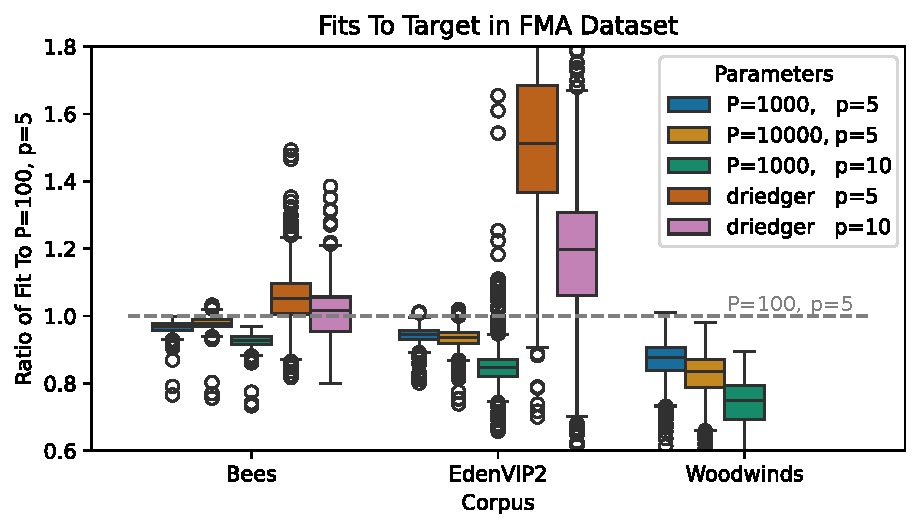
\includegraphics[width=\columnwidth]{figs/FMAFit.pdf}
    \caption{Increasing polyphony leads to a better fit (ratios $<1$), and increasing particles leads to a better fit, especially for larger corpora like the Woodwinds ($\approx$1.6hrs).}
    \label{fig:fmafit}
\end{figure}

First, we assess the effect of particles on fit; we fix $p_d=0.95$, temperature=10, and $r=3$, using $L=10$ iterations for all KL operations, and we take $P \in \left\{ 100, 1000, 10000 \right\}$.  We also compare to Driedger et. al's technique with $c=3$ and $r=3$ using $L=50$ iterations, though we omit results on Woodwinds due to computational cost (Section~\ref{sec:complexity}).  In all cases, we use frequencies from $0$ to $8000$hz using a sample rate of 44100hz, a window length of 2048 samples, and a hop length of 1024 samples.  Since the spectral similarity of different targets to a particular corpus varies widely, we report the {\em ratio} of the KL loss in Equation~\ref{eq:klloss} to the KL loss for The Concatenator with $P=100, p=5$.  Figure~\ref{fig:fmafit} shows the results.  As expected, an increased polyphony leads to a better fit, as does increasing particles for all but the Bees, though the effect of increased particles is most pronounced for the largest corpus of Woodwinds, which makes sense by Equation~\ref{eq:timeadjacentprobmodified}.


\begin{figure}
    \centering
    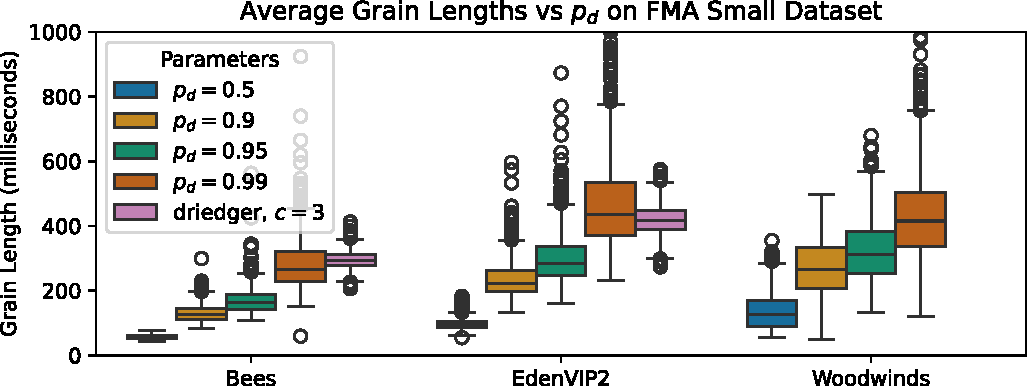
\includegraphics[width=\columnwidth]{figs/pdGrainLengths.pdf}
    \caption{Increasing $p_d$ increases the average grain length since activations are less likely to jump at each timestep.}
    \label{fig:pdGrainLengths}
\end{figure}


\begin{figure}
    \centering
    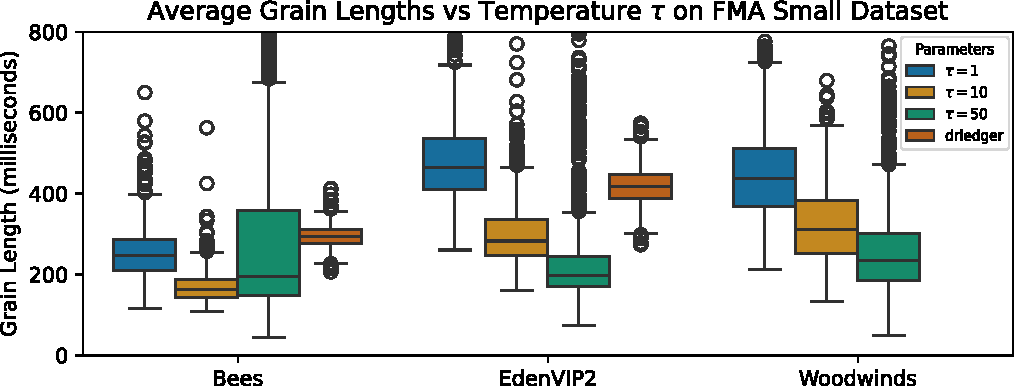
\includegraphics[width=\columnwidth]{figs/tempGrainLengths.pdf}
    \caption{Increasing $\tau$ {\em decreases} the average grain length since this prioritizes the observation probability.}
    \label{fig:tempGrainLengths}
\end{figure}

As we noted in Section~\ref{sec:relatedwork}, however, a very good fit may lose the timbral characteristics of the corpus.  This is mitigated by a low $p$, but we also need to ensure that grains are long enough.  Therefore, we also examine mean grain length for various parameters.  Figure~\ref{fig:pdGrainLengths} shows the result of varying $p_d$ for a fixed temperature $\tau=10$ and $p=5$, and Figure~\ref{fig:tempGrainLengths} shows the result of varying the temperature $\tau$ for $p=5$ and $p_d = 0.95$.  As expected, grain length goes up with an increase $p_d$ and down with an increase in $\tau$.  In practice, lowering $\tau$ and raising $p_d$ will lead to especially long grain lengths, while possibly losing an acceptable fit to the target.


\textbf{Reproducing Pitch.} How well does The Concatenator reproduce target pitch?


%\begin{figure}
%    \centering
%    \includegraphics[width=0.7\textwidth]{figs/PitchEstimates.png}
%    \caption{Pitch estimates}
%    \label{fig:pitchestimates}
%\end{figure}


\subsection{Qualitative Evaluation}

Talk about Ben's ``obstacle course''

\subsection{Discussion}

Randomness is an asset

The obstacle course doesn't necessarily tell us where the model can go

We also believe the formulation of this particle filter opens up other approaches to MIR such as real time multipitch tracking, structure analysis of large scale audio, and sample detection.

% For bibtex users:
\bibliography{ISMIRtemplate}

% For non bibtex users:
%\begin{thebibliography}{citations}
% \bibitem{Author:17}
% E.~Author and B.~Authour, ``The title of the conference paper,'' in {\em Proc.
% of the Int. Society for Music Information Retrieval Conf.}, (Suzhou, China),
% pp.~111--117, 2017.
%
% \bibitem{Someone:10}
% A.~Someone, B.~Someone, and C.~Someone, ``The title of the journal paper,''
%  {\em Journal of New Music Research}, vol.~A, pp.~111--222, September 2010.
%
% \bibitem{Person:20}
% O.~Person, {\em Title of the Book}.
% \newblock Montr\'{e}al, Canada: McGill-Queen's University Press, 2021.
%
% \bibitem{Person:09}
% F.~Person and S.~Person, ``Title of a chapter this book,'' in {\em A Book
% Containing Delightful Chapters} (A.~G. Editor, ed.), pp.~58--102, Tokyo,
% Japan: The Publisher, 2009.
%
%
%\end{thebibliography}

\end{document}

